\section{Accuracy}
\label{sec:accuracy}

\citep{Mitchell97} provides succinct definition:
\begin{quote}
    A computer program is said to learn from experience $E$ with respect to
    some class of tasks $T$ and performance measure $P$, if its performance
    at tasks in $T$, as measured by $P$, improves with experience $E$.
\end{quote}
And for the most supervised machine learning tasks, the accuracy(Eq.\ref{eq:accuracy}), or say error-rate(Eq.\ref{eq:error-rate})
is used as the simplest evaluation.
\begin{eqnarray}
    \label{eq:accuracy}
    A = \frac{n_{right}}{n} \\
    \label{eq:error-rate}
    E = \frac{n_{error}}{n}
\end{eqnarray}
We use the accuracy on testing set to evaluate the model.
The most common way is to splitting the testing set from the dataset randomly,
and then testing the model with testing set.
Moreover, the accuracy is also the simple the loss function $\ell$, or say cost function.
Back to the accuracy, it can not be used to evaluate model sometimes. The following section will
give an example.

\section{Four Kind of Results}
\label{sec:4rt}

This section will be based on a problem about 2-class classification.
There is a line,  $ax+by+c = 0$, split a 2-D space into two area.
One of the area is labeled with $\oplus$(positive), while other area is labeled with $\ominus$(negative).
In the Fig.\ref{fig:classification-1}, the red points should be labeled with $\ominus$, while
the blue ones should be labeled with $\oplus$.
Function $f(\cdot)$ is model learned in someways to classify. When $f(x,y) > 0$ satisfied,
point $(x,y)$ is above the line.
\begin{figure}
    \centering
    \begin{tikzpicture}
    \begin{axis}[axis lines=middle, xmin=-2, xmax=2,ymin=-4.5, ymax=2,xlabel=$x$, ylabel=$y$]
        \addplot[domain=-2:2] {2*x-1};
        \addplot[only marks,color=blue] coordinates {
            (1,-2)
            (-0.2,-3.5)
            (1.5,0.3)
        };
        \addplot[only marks,color=red] coordinates {
            (0.4,0.8)
            (-1.5,-1)
            (-1.3,0.4)
        };
    \end{axis}
    \end{tikzpicture}
    \caption{Classification.}
    \label{fig:classification-1}
\end{figure}

Let's assume $f(\cdot)$ defined as $f(x) = \overline{a}x+\overline{b}y+\overline{c}$,
just like the red line in Fig.\ref{fig:classification-2}.
The blue and green points are marked to positive by $f(\cdot)$, while the pink and red points are
marked to negative. However, the pink and blue points belong to positive class, while
the red and green points belong to negative class.

So there are four kinds of results are ``true positive'', ``false positive'', ``true negative'',
and ``false negative'' corresponding to {\color{blue}blue points}, {\color{green}green points},
{\color{red}red points}, and {\color{pink}pink points}.



\begin{figure}
    \centering
    \begin{tikzpicture}
    \begin{axis}[axis lines=middle, xmin=-2, xmax=2,ymin=-4.5, ymax=2,xlabel=$x$, ylabel=$y$]
    \addplot[domain=-2:2] {2*x-1};
    \addplot[domain=-2:2,color=red] {-2*x-1};
    \addplot[only marks,color=blue] coordinates {
        (1,-2)
        (1.5,0.3)
    };
    \addplot[only marks,color=red] coordinates {
        (-1.5,-1)
        (-1.3,0.4)
    };
    \addplot[only marks,color=green] coordinates {
        (0.4,0.8)
        (-0.6,0.456)
    };
    \addplot[only marks,color=pink] coordinates {
        (0.3,-4)
        (-0.2,-3.5)
    };
    \end{axis}
    \end{tikzpicture}
    \caption{Classification with model}
    \label{fig:classification-2}
\end{figure}

Then 8 variables can be defined, Tab.\ref{tab:8v}.

\begin{table}
    \centering
\begin{tabular}{cc}
    \hline
    $n_{tp}$ & the number of ``true positive'' \\ 
    $n_{fp}$ & the number of ``false positive'' \\ 
    $n_{tn}$ & the number of ``true negative'' \\ 
    $n_{fn}$ & the number of ``false negative'' \\ 
    $r_{tp}$, $r$ & recall, ratio of $n_{tp}$ and $n_{tp} + n_{fn}$ \\ 
    $r_{fp}$ & the ratio of $n_{fp}$ and $n_{fp} + n_{tn}$ \\ 
    $p$ &  precision, ratio of $n_{tp}$ and $n_{tp} + n_{fp}$ \\ 
    $f^{(1)}$ & F1-score. $\frac{2pr}{p+r}$ \\ 
    \hline 
\end{tabular}
`   \caption{Eight variables}
\label{tab:8v}
\end{table}

\subsection{The condition that accuracy loss efficacy}
\label{sec:4rt:eg}

When we test the model $f(\cdot)$ in Fig.\ref{fig:classification-2} with the test set which is not enough random,
for example, the points in blue are over more than points in green,
the accuracy, or say precision $p$ might be good enough, but is the model good enough?

\section{Precision and Recall}
\label{sec:pr}

Precision $p$ is defined as $\frac{n_{tp}}{n_{tp} + n_{fp}}$, while recall $r$ is defined
as $\frac{n_{tp}}{n_{tp} + n_{fn}}$. The former means the $p$ of items labeled with positive
by model are the real positive, while the latter means the $r$ of positive items are labeled
by model with positive.

The larger precision $p$ and recall $r$ are ,the model is better.

\section{Precision Recall Curve}
\label{sec:prc}

Precision Recall Curve is a curve to describe the relationship between $p$ and $r$ of a model.
For the task which missing positive item is better than recognizing negative item as positive,
the recall $r$ will be more important. For the task which negative item is better than
recognizing missing positive item as positive, the recall $p$ will be more important.
\begin{figure}
    \centering
    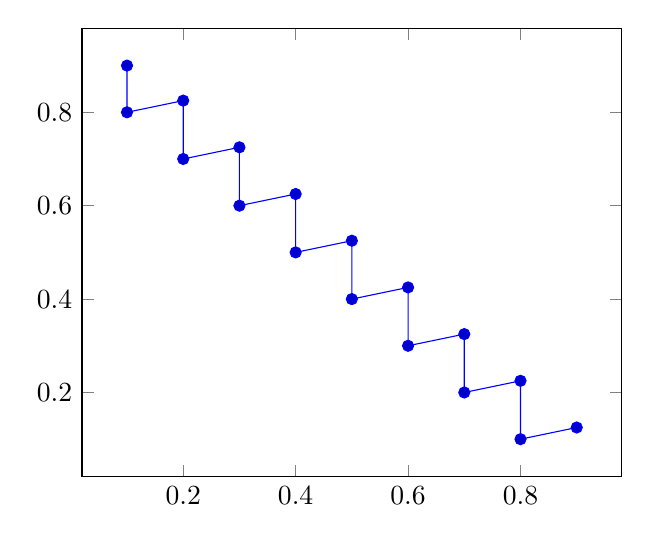
\begin{tikzpicture}
    \begin{axis}
        \addplot coordinates {
            (0.1,0.9)
            (0.1,0.8)
            (0.2,0.825)
            (0.2,0.7)
            (0.3,0.725)
            (0.3,0.6)
            (0.4,0.625)
            (0.4,0.5)
            (0.5,0.525)
            (0.5,0.4)
            (0.6,0.425)
            (0.6,0.3)
            (0.7,0.325)
            (0.7,0.2)
            (0.8,0.225)
            (0.8,0.1)
            (0.9,0.125)
        };
    \end{axis}
    \end{tikzpicture}
    \caption{Precision Recall Curve}
    \label{fig:prc-1}
\end{figure}
The more smooth the curve is, the model is better,
The larger area under curve, AUC for short, is, the model is better.
When $p$ and $r$ are closer to $1.0$, the AUC will be larger.
        
\section{F1-score}
\label{sec:f1-s}

F1-score is a value to measure the performance of a model.
The larger $f^{(1)}$ is, and the model is better.
The Fig.\ref{fig:classification-2} shows that when the line of model $f(\cdot)$ is more coincident
with line $ax+by+c=0$, the $p$ and $r$ are closer to $1.0$,
and then f1-score $f^{(1)}$ will be larger.

F1-score is a particular case of ``Fa-score'' defined as Eq.\ref{eq:fa-s}.
\begin{equation}
    \label{eq:fa-s}
    F^{(\alpha)} = \frac{\left(\alpha^2+1\right)pr}{\alpha^2p + r}
\end{equation}

\section{Receiver Operating Characteristic Curve}
\label{sec:roc}

Receiver operating characteristic curve(Fig.\ref{fig:roc},red curve), ROC for short, is another performance measure.
One axis of ROC is $r_{tp}$, or say recall $r$, while other axis is $r_{fp}$.
\begin{figure}
    \centering
    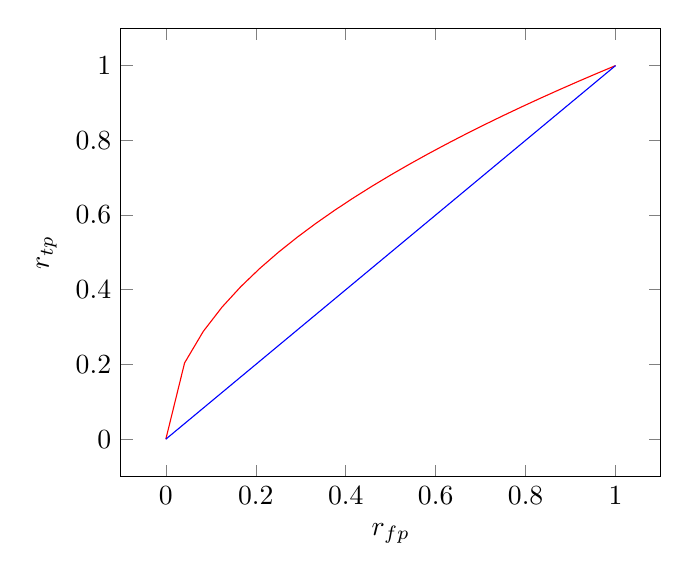
\begin{tikzpicture}
    \begin{axis}[xlabel=$r_{fp}$, ylabel=$r_{tp}$]
        \addplot[domain=0:1,color=red] {sqrt(x)};
        \addplot[domain=0:1,color=blue] {x};
    \end{axis}
    \end{tikzpicture}
    \caption{Receiver Operating Characteristic Curve}
    \label{fig:roc}
\end{figure}
The more smooth ROC is, the model is better, while the larger
receiver operating characteristic curve area under curve, ROC-AUC for short, is,
the model is better.

More, when the ROC is not above of $y=x$, the model will performance worth than a random number,
or say a random classifier.

\section{Kolmogorov-Simrnov Score}
\label{sec:ks-c}

The Kolmogorov-Simrnov score, KS for short is defined as Eq.\ref{eq:ks-c}.
\begin{equation}
    \label{eq:ks-c}
    KS = \max\left(r_{tp} - r_{fp}\right)
\end{equation}
KS can be used to measure the performance in telling the difference between positive and negative.
The best hyper-parameters $\theta$ of a model will be $\arg\max f(x;\theta)$.

\bibliography{../../random-bib/deep-learning%
                ,../../random-bib/machine-learning%
}
\bibliographystyle{plainnat}